\documentclass[../distribution_theory_notes.tex]{subfiles}
\begin{document}
\section{Aula 21 - 08 de Novembro, 2024}
\subsection{Motivações}
\begin{itemize}
	\item Densidade das funções teste em \(\mathcal{D}'(\Omega )\) na topologia fraca-*;
	\item Propriedades de suporte para convoluções e produtos;
	\item Estrutura local das distribuições.
\end{itemize}
\subsection{Preparação para a Densidade e a Estrutura Local}
Na aula passada, demonstramos um dos resultados mais impressionantes deste curso: para uma distribuição \(u\in \mathcal{D}'(\mathbb{R}^{n})\),
\[
	\mathrm{supp}(u)=\{0\}\quad\Longleftrightarrow\quad u=\sum\limits_{| \alpha  |\leq m}^{}a_{\alpha }\partial^{\alpha }\delta,
\]
para certos coeficientes \(a_{\alpha }\in \mathbb{C}\), com \(| \alpha  |\leq m\). Num certo sentido, o suporte caracteriza a forma que a distribuição assume.

A demonstração deste resultado revela, mais uma vez, que todo o problema é transferido para propriedades das funções teste. Em particular, foram indispensáveis alguns dos seguintes pontos-chave:
\begin{itemize}
	\item[(i)] a Fórmula de Taylor com resto integral expressa em notação de multi-índices;
	\item[(ii)] a independência da função de Urysohn \(\psi \) associada a \(K=\mathrm{supp}(u)\), quando K é compacto, para a avaliação
	      \[
		      \langle u, \varphi  \rangle=\langle u, \psi \varphi  \rangle,
	      \]
	      para toda \(\varphi \) apropriada;
	\item[(iii)] o modo como se constrói uma função de Urysohn por meio da convolução com uma família regularizante \((\varphi_{\varepsilon })_{\varepsilon >0}\); e
	\item[(iv)] as estimativas que uma \(u\in \mathcal{E}'(\Omega )\) deve satisfazer.
\end{itemize}

Nosso objetivo é reunir alguns fatos já aprendidos sobre distribuições e localizações para ampliar o alcance de resultados anteriores. Em particular, demonstraremos a densidade de \(\mathcal{C}_{c}^{\infty}(\Omega )\) em \(\mathcal{D}'(\Omega )\), na topologia fraca-*, para um aberto qualquer \(\Omega \subseteq \mathbb{R}^{n}\). Também explicitaremos um argumento usado na prova do teorema da aula passada, relacionado ao item (iv): a uniformidade da constante \(c>0\) e da ordem de derivação m nas estimativas, independentemente de \(\varepsilon >0\).

Por fim, encerraremos esta introdução ao conceito de localização demonstrando o Teorema de Estrutura Local das Distribuições, segundo o qual, dados \(u\in \mathcal{D}'(\Omega )\) e um aberto limitado \(U\subseteq \Omega \) com \(\overline{U}\subseteq \Omega \), existem \(\alpha \in \mathbb{Z}_{+}^{n}\) e \(f\in \mathcal{C}(\overline{U})\) tais que
\[
	\partial^{\alpha }f=u\quad\text{em }\mathcal{D}'(U).
\]
Em outras palavras, toda distribuição é, localmente, a derivada de alguma ordem de uma função contínua (chocante!). Os próximos passos também preparam o terreno para a Parte III do produto de convolução ``\(u*v\)'', na qual ambos os fatores serão distribuições.

\begin{tcolorbox}[
		skin=enhanced,
		title=Observação,
		fonttitle=\bfseries,
		colframe=black,
		colbacktitle=cyan!75!white,
		colback=cyan!15,
		colbacklower=black,
		coltitle=black,
		drop fuzzy shadow,
		%drop large lifted shadow
	]
	Seja \(u\in \mathcal{D}'(\Omega )\) com \(K=\mathrm{supp}(u)\) compacto. Se fixarmos \(\Psi \in \mathcal{C}_{c}^{\infty}(\Omega )\) uma função de Urysohn associada a K e pusermos \(K_{0}\coloneqq \mathrm{supp}(\Psi )\), existem \(M>0\) e \(m\in \mathbb{Z}_{+}\) tais que
	\[
		| \langle \overline{u}, f \rangle |\leq M\sum\limits_{| \alpha  |\leq m}^{}\sup_{x\in K_{0}}| \partial^{\alpha }f(x) |,
		\quad \forall f\in \mathcal{C}^{\infty}(\Omega ),
	\]
	onde \(\overline{u}\) é a única extensão de u a \(\mathcal{C}^{\infty}(\Omega )\), conforme a segunda parte da identificação
	\[
		\mathcal{D}'_{c}(\Omega )=\mathcal{E}'(\Omega ).
	\]
	Essa estimativa, em particular, confirma que \(\overline{u}\in \mathcal{E}'(\Omega )\).

	Além disso, se \(\psi_{0}\in \mathcal{C}_{c}^{\infty}(\Omega )\) é qualquer função que satisfaz \(\psi_{0}\equiv 1\) numa vizinhança de \(K=\mathrm{supp}(u)\), então
	\[
		\langle u, \varphi  \rangle=\langle u, \psi_{0}\varphi  \rangle,
	\]
	para toda \(\varphi \in \mathcal{C}_{c}^{\infty}(\Omega )\), e a mesma expressão vale para toda \(\varphi \in \mathcal{C}^{\infty}(\Omega )\) quando calculamos \(\overline{u}\).

	Desta maneira, qualquer que seja \(\varphi \in \mathcal{C}_{c}^{\infty}(\Omega )\), vale
	\begin{align*}
		| \langle u, \varphi  \rangle | & \leq M\sum\limits_{| \alpha  |\leq m}^{}\sup_{x\in K_{0}}| \partial^{\alpha }\varphi (x) |           \\
		                                & \leq M\sum\limits_{| \alpha  |\leq m}^{}\sup_{x\in \mathbb{R}^{n}}| \partial^{\alpha }\varphi (x) |.
	\end{align*}
	Isso mostra não apenas que u é de ordem finita, menor ou igual a m, mas também que a constante M das estimativas necessárias para que u seja distribuição independe do compacto \(K'\subseteq \Omega \) que suporta as funções teste.

	Esta observação torna o m e o \(c>0\) usados na prova do teorema da aula passada independentes de \(\varepsilon >0\). Uma outra maneira seria fixar \(K'=\overline{B}(0;1)\) e usar a estimativa associada a ele; ambas as maneiras são válidas, mas a segunda deixa a demonstração contida em si mesma.
\end{tcolorbox}

\subsection{Densidade das Funções Teste em \(\mathcal{D}'(\Omega )\)}
Começamos com dois lemas sobre suporte, o primeiro dos quais também será útil em situações futuras envolvendo convoluções.

\begin{lemma*}
	Se \(u\in \mathcal{D}'(\mathbb{R}^{n})\) e \(\varphi \in \mathcal{C}_{c}^{\infty}(\mathbb{R}^{n})\), então
	\[
		\mathrm{supp}(u*\varphi )\subseteq \mathrm{supp}(u)+\mathrm{supp}(\varphi ).
	\]
\end{lemma*}
\begin{proof*}
	Primeiramente, lembremos que, para todo \(x\in \mathbb{R}^{n}\),
	\[
		u*\varphi (x)=\langle u, \tau_{x}\check{\varphi } \rangle.
	\]
	Consequentemente, se
	\[
		\mathrm{supp}(\tau_{x}\check{\varphi })\cap \mathrm{supp}(u)=\emptyset,
	\]
	então \(u*\varphi (x)=0\), de acordo com a definição do suporte de u.

	Pensando nisso, basta encontrarmos condições sobre x em \(\mathbb{R}^{n}\) para que os suportes de \(\tau_{x}\check{\varphi }\) e \(u\) sejam disjuntos. Como
	\[
		\mathrm{supp}(\tau_{x}\check{\varphi })=x-\mathrm{supp}(\varphi ),
	\]
	temos
	\begin{align*}
		\mathrm{supp}(\tau_{x}\check{\varphi })\cap \mathrm{supp}(u)\neq \emptyset
		 & \Longleftrightarrow (x-\mathrm{supp}(\varphi ))\cap \mathrm{supp}(u)\neq \emptyset         \\
		 & \Longleftrightarrow \exists z\in \mathrm{supp}(\varphi ),\; y\in \mathrm{supp}(u):\; y=x-z \\
		 & \Longleftrightarrow x=y+z,\quad y\in \mathrm{supp}(u),\; z\in \mathrm{supp}(\varphi )      \\
		 & \Longleftrightarrow x\in \mathrm{supp}(u)+\mathrm{supp}(\varphi ).
	\end{align*}
	Logo,
	\[
		x\notin \mathrm{supp}(u)+\mathrm{supp}(\varphi )
		\Longrightarrow u*\varphi (x)=0.
	\]
	Portanto,
	\[
		\mathrm{supp}(u*\varphi )\subseteq \overline{\mathrm{supp}(u)+\mathrm{supp}(\varphi )}
		=\mathrm{supp}(u)+\mathrm{supp}(\varphi ),
	\]
	pois \(\mathrm{supp}(u)\) é fechado e \(\mathrm{supp}(\varphi )\) é compacto. \qedsymbol
\end{proof*}

Vale a pena, neste momento, demonstrar também o seguinte resultado.
\begin{lemma*}
	Se \(f\in \mathcal{C}^{\infty}(\Omega )\) e \(u\in \mathcal{D}'(\Omega )\), então
	\[
		\mathrm{supp}(fu)\subseteq \mathrm{supp}(f)\cap \mathrm{supp}(u).
	\]
\end{lemma*}
\begin{proof*}
	Por um lado, se \(\varphi \in \mathcal{C}_{c}^{\infty}(\Omega \setminus{\mathrm{supp}(f)})\), então \(\varphi f=0\) em \(\Omega \), de maneira que
	\[
		\langle fu, \varphi  \rangle=\langle u, f\varphi  \rangle=0.
	\]
	Assim,
	\[
		fu|_{\Omega \setminus{\mathrm{supp}(f)}}=0
		\quad\Longrightarrow\quad
		\mathrm{supp}(fu)\subseteq \mathrm{supp}(f).
	\]

	Por outro lado, se \(\varphi \in \mathcal{C}_{c}^{\infty}(\Omega \setminus{\mathrm{supp}(u)})\), então
	\[
		\mathrm{supp}(f\varphi )\subseteq \mathrm{supp}(f)\cap \mathrm{supp}(\varphi )\subseteq \mathrm{supp}(\varphi ),
	\]
	e, portanto,
	\[
		\mathrm{supp}(f\varphi )\cap \mathrm{supp}(u)=\emptyset
		\Longrightarrow
		\langle fu, \varphi  \rangle=\langle u, f\varphi  \rangle=0.
	\]
	Consequentemente,
	\[
		fu|_{\Omega \setminus{\mathrm{supp}(u)}}=0
		\quad\Longrightarrow\quad
		\mathrm{supp}(fu)\subseteq \mathrm{supp}(u).
	\]
	Em resumo,
	\[
		\mathrm{supp}(fu)\subseteq \mathrm{supp}(f)\cap \mathrm{supp}(u).\text{ \qedsymbol}
	\]
\end{proof*}

Agora já não falta mais nada para a densidade desejada.
\begin{theorem*}
	Seja \(\Omega \subseteq \mathbb{R}^{n}\) um aberto qualquer. Então \(\mathcal{C}_{c}^{\infty}(\Omega )\) é fraco-* denso em \(\mathcal{D}'(\Omega )\).
\end{theorem*}
\begin{proof*}
	Em primeiro lugar, \(\mathcal{E}'(\Omega )\) é denso em \(\mathcal{D}'(\Omega )\). Com efeito, seja \(u\in \mathcal{D}'(\Omega )\), seja \((K_{j})_{j\in \mathbb{N}}\) um esgotamento de \(\Omega \) e, para cada j, seja \(\psi_{j}\in \mathcal{C}_{c}^{\infty}(\Omega )\) uma função de Urysohn associada ao compacto \(K_{j}\); então, para toda \(\varphi \in \mathcal{C}_{c}^{\infty}(\Omega )\),
	\[
		\psi_{j}\varphi \stackrel{j\to \infty}{\longrightarrow}\varphi
		\quad\text{em }\mathcal{C}_{c}^{\infty}(\Omega ),
	\]
	por conseguinte,
	\[
		\langle \psi_{j}u, \varphi  \rangle
		=\langle u, \psi_{j}\varphi  \rangle
		\stackrel{j\to \infty}{\longrightarrow}
		\langle u, \varphi  \rangle.
	\]
	Pelo lema anterior,
	\[
		\mathrm{supp}(\psi_{j}u)\subseteq \mathrm{supp}(\psi_{j})\cap \mathrm{supp}(u)\subseteq \mathrm{supp}(\psi_{j}),
	\]
	e este último conjunto é compacto. Portanto, \(\psi_{j}u\in \mathcal{E}'(\Omega )\) para todo j, provando a primeira afirmação.

	Em segundo lugar, \(\mathcal{C}_{c}^{\infty}(\Omega )\) é denso em \(\mathcal{E}'(\Omega )\). De fato, se \(u\in \mathcal{E}'(\Omega )\) é qualquer, então u é, na realidade, a restrição a \(\Omega \) de uma distribuição \(\overline{u}\in \mathcal{D}'(\mathbb{R}^{n})\), não necessariamente única. Para obter uma tal extensão, basta escolher \(\psi \in \mathcal{C}_{c}^{\infty}(\Omega )\) uma função de Urysohn associada a \(\mathrm{supp}(u)\) e definir
	\[
		\langle \overline{u}, f \rangle\coloneqq \langle u, \psi f \rangle,
		\quad f\in \mathcal{C}_{c}^{\infty}(\mathbb{R}^{n}).
	\]
	Decorre do que já foi feito na identificação \(\mathcal{E}'=\mathcal{D}'_{c}\) que \(\overline{u}\) está bem definida independentemente da escolha de \(\psi \), que \(\overline{u}\) tem suporte compacto igual a \(\mathrm{supp}(u)\) e que
	\[
		\overline{u}|_{\Omega }=u.
	\]

	Nessas condições, se \((\varphi_{\varepsilon })_{\varepsilon >0}\) é uma família regularizante padrão e \(\phi \in \mathcal{C}_{c}^{\infty}(\mathbb{R}^{n})\), então
	\begin{align*}
		\langle \overline{u}*\varphi_{\varepsilon }, \phi  \rangle
		 & =[(\overline{u}*\varphi_{\varepsilon })*\check{\phi}](0)                        \\
		 & =[\overline{u}*(\varphi_{\varepsilon }*\check{\phi})](0)                        \\
		 & =\langle \overline{u}, (\varphi_{\varepsilon }*\check{\phi})^{\check{}} \rangle
		\stackrel{\varepsilon \to 0^{+}}{\longrightarrow}\langle \overline{u}, \phi  \rangle,
	\end{align*}
	pois \(\varphi_{\varepsilon }*\eta \to \eta \) em \(\mathcal{C}_{c}^{\infty}\) quando \(\varepsilon \to 0^{+}\), para toda \(\eta \in \mathcal{C}_{c}^{\infty}\). Em particular,
	\[
		(\overline{u}*\varphi_{\varepsilon })|_{\Omega }
		\stackrel{\varepsilon \to 0^{+}}{\longrightarrow}
		\overline{u}|_{\Omega }=u
	\]
	na topologia fraca-* de \(\mathcal{D}'(\Omega )\).

	Finalmente, pelo primeiro lema,
	\[
		\mathrm{supp}(\overline{u}*\varphi_{\varepsilon })
		\subseteq \mathrm{supp}(\overline{u})+\overline{B}(0;\varepsilon )
		=\mathrm{supp}(u)+\overline{B}(0;\varepsilon ).
	\]
	Como
	\[
		0<\varepsilon <d(\mathrm{supp}(u),\mathbb{R}^{n}\setminus \Omega )
	\]
	implica
	\[
		\mathrm{supp}(u)+\overline{B}(0;\varepsilon )\subseteq \Omega,
	\]
	segue que \(\mathrm{supp}(\overline{u}*\varphi_{\varepsilon })\) é compacto em \(\Omega \) para \(\varepsilon >0\) suficientemente pequeno. Como \(\overline{u}*\varphi_{\varepsilon }\in \mathcal{C}^{\infty}\), concluímos que
	\[
		\overline{u}*\varphi_{\varepsilon }\in \mathcal{C}_{c}^{\infty}(\Omega )
	\]
	para \(\varepsilon \) pequeno. Juntando esta afirmação à densidade de \(\mathcal{E}'(\Omega )\) em \(\mathcal{D}'(\Omega )\), o teorema está provado. \qedsymbol
\end{proof*}

\subsection{Estrutura Local das Distribuições}
Queremos demonstrar que, dados \(\Omega \subseteq \mathbb{R}^{n}\) aberto, \(u\in \mathcal{D}'(\Omega )\) e \(U\subseteq \Omega \) um aberto limitado com \(\overline{U}\subseteq \Omega \), existem \(f\in \mathcal{C}(\overline{U})\) e \(\alpha \in \mathbb{Z}_{+}^{n}\) tais que
\[
	\partial^{\alpha }f=u\quad\text{em }\mathcal{D}'(U).
\]
O ponto-chave da demonstração consiste em estabelecer uma estimativa elementar para funções teste.
\begin{figure}[H]
	\begin{center}
		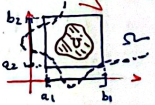
\includegraphics[height=0.3\textheight, width=0.3\textwidth, keepaspectratio]{./Images/21_small.png}
	\end{center}
\end{figure}

Suponhamos que
\[
	U\subseteq \prod_{i=1}^{n}[a_{i},b_{i}].
\]
Então, para toda \(\psi \in \mathcal{C}_{c}^{\infty}(\overline{U})\) e todo \(m\in \mathbb{N}\), vale
\[
	\sup | \psi (x) |
	\leq (b_{1}-a_{1})^{m}(b_{2}-a_{2})^{m}\cdots (b_{n}-a_{n})^{m}
	\sup | \partial_{1}^{m}\partial_{2}^{m}\cdots \partial_{n}^{m}\psi (x) |. \tag{*}
\]
Com efeito, por aplicações sucessivas do Teorema Fundamental do Cálculo, para qualquer \(1\leq j\leq n\),
\[
	\psi (x)=\int_{a_{j}}^{x_{j}}
	\frac{\partial \psi }{\partial x_{j}}(x_{1},\dotsc ,t,\dotsc ,x_{n})\,\mathrm{d}t,
\]
pois \(\psi \) tem suporte compacto no retângulo considerado. Logo,
\[
	| \psi (x) |\leq (b_{j}-a_{j})\sup_{z\in \mathbb{R}^{n}}\biggl| \frac{\partial \psi }{\partial x_{j}}(z)\biggr|.
\]
Aplicando novamente o mesmo argumento à derivada \(\partial \psi /\partial x_{j}\), obtemos
\[
	\sup | \psi (x) |\leq (b_{j}-a_{j})^{2}\sup_{z\in \mathbb{R}^{n}}\biggl| \frac{\partial^{2}\psi }{\partial x_{j}^{2}}(z)\biggr|,
\]
e, sucessivamente,
\[
	\sup | \psi (x) |\leq (b_{j}-a_{j})^{m}\sup | \partial_{j}^{m}\psi (x) |. \tag{I}
\]
Aplicando (I) primeiro com \(j=1\), depois com \(j=2\) à função \(\partial_{1}^{m}\psi \), e assim sucessivamente até \(j=n\), obtém-se (*).

\begin{tcolorbox}[
		skin=enhanced,
		title=Observação,
		fonttitle=\bfseries,
		colframe=black,
		colbacktitle=cyan!75!white,
		colback=cyan!15,
		colbacklower=black,
		coltitle=black,
		drop fuzzy shadow,
		%drop large lifted shadow
	]
	Um problema bem mais difícil seria provar uma desigualdade de sentido contrário, isto é, dominar as derivadas de \(\psi \) pela própria \(\psi \). Lembre-se das estimativas de Cauchy para funções holomorfas e, analogamente, para funções harmônicas.
\end{tcolorbox}

Agora, dada \(u\in \mathcal{D}'(\Omega )\) e seja \(U\subseteq \Omega \) um aberto limitado com \(\overline{U}\subseteq \Omega \). Associados ao compacto \(K=\overline{U}\), existem \(c>0\) e \(r\in \mathbb{Z}_{+}\) tais que
\[
	| \langle u, \phi  \rangle |
	\leq c\sum\limits_{| \alpha  |\leq r}^{}\sup | \partial^{\alpha }\phi (x) |,
	\quad \forall \phi \in \mathcal{C}_{c}^{\infty}(\overline{U}).
\]
Escrevendo
\begin{align*}
	\sum\limits_{| \alpha  |\leq r}^{}\sup_{}| \partial^{\alpha }\varphi  | & = \sum\limits_{i=0}^{r}\sum\limits_{| \alpha  |=i}^{}\sup_{}| \partial^{\alpha }\varphi  |                                                                           \\
	                                                                        & = \sup_{}| \varphi  |+\sum\limits_{k=1}^{n}\sup_{}| \partial_{k}\varphi  | + \sum\limits_{j=1}^{n}\sum\limits_{k=1}^{n}\sup_{}| \partial_{j}\partial_{k}\varphi  | + \\
	                                                                        & \quad +\dotsc + \sum\limits_{| \alpha  |=r}^{}\sup_{}| \partial_{1}^{\alpha_1}\partial_{2}^{\alpha_2}\dotsc \partial_{n}^{\alpha_{n}}\varphi  |
\end{align*}
e escolhendo um retângulo \(\prod_{i=1}^{n}[a_{i},b_{i}]\) que contém U, podemos usar (*) para estimar cada parcela da soma acima, completando os expoentes até a ordem máxima \(m=r\). Assim,
\begin{align*}
	 & \sup | \phi |  \leq c_{0}\sup | \partial_{1}^{r}\partial_{2}^{r}\cdots \partial_{n}^{r}\phi |,
	\quad c_{0}=(b_{1}-a_{1})^{r}\cdots (b_{n}-a_{n})^{r},                                            \\
	 & \sup | \partial_{k}\phi |
	\leq (b_{1}-a_{1})^{r}\cdots (b_{k}-a_{k})^{r-1}\cdots (b_{n}-a_{n})^{r}
	\sup | \partial_{1}^{r}\cdots \partial_{n}^{r}\phi |,                                             \\
	 & \sup | \partial_{k}\partial_{j}\phi |
	\leq (b_{1}-a_{1})^{r}\cdots (b_{k}-a_{k})^{r-1}\cdots (b_{j}-a_{j})^{r-1}\cdots (b_{n}-a_{n})^{r}
	\sup | \partial_{1}^{r}\cdots \partial_{n}^{r}\phi |,
\end{align*}
e, de modo geral, para \(\alpha = (\alpha_{1},\dotsc ,\alpha_{n})\) com \(| \alpha  |\leq r\),
\[
	\sup | \partial_{1}^{\alpha_{1}}\partial_{2}^{\alpha_{2}}\cdots \partial_{n}^{\alpha_{n}}\phi |
	\leq \prod_{i=1}^{n}(b_{i}-a_{i})^{r-\alpha_{i}}
	\sup | \partial_{1}^{r}\partial_{2}^{r}\cdots \partial_{n}^{r}\phi |.
\]
Consequentemente, existe \(c'>0\), dependendo apenas de U, da ordem r e da dimensão n, tal que
\[
	| \langle u, \phi  \rangle |
	\leq c'\sup | \partial_{1}^{r}\partial_{2}^{r}\cdots \partial_{n}^{r}\phi (x) |,
	\quad \forall \phi \in \mathcal{C}_{c}^{\infty}(\overline{U}). \tag{**}
\]

Por outro lado, o Teorema Fundamental do Cálculo, mais uma vez, fornece
\[
	\partial_{1}^{r}\partial_{2}^{r}\cdots \partial_{n}^{r}\phi (x)
	=\int_{A_{x}}^{}
	\partial_{1}^{r+1}\partial_{2}^{r+1}\cdots \partial_{n}^{r+1}\phi (y)\,\mathrm{d}y,
\]
onde
\[
	A_{x}\coloneqq \{y\in \mathbb{R}^{n}:y_{j}\leq x_{j},\; j=1,2,\dotsc ,n\}.
\]
Daí,
\begin{align*}
	| \partial_{1}^{r}\cdots \partial_{n}^{r}\phi (x) |
	 & \leq \int_{A_{x}}^{}| \partial_{1}^{r+1}\cdots \partial_{n}^{r+1}\phi (y) |\,\mathrm{d}y           \\
	 & \leq \int_{\mathbb{R}^{n}}^{}| \partial_{1}^{r+1}\cdots \partial_{n}^{r+1}\phi (y) |\,\mathrm{d}y,
\end{align*}
de modo que
\[
	\sup | \partial_{1}^{r}\cdots \partial_{n}^{r}\phi (x) |
	\leq \| \partial_{1}^{r+1}\cdots \partial_{n}^{r+1}\phi \|_{L^{1}}.
\]
Juntando esta estimativa com (**), obtemos
\[
	| \langle u, \phi  \rangle |
	\leq c'\| \partial_{1}^{r+1}\partial_{2}^{r+1}\cdots \partial_{n}^{r+1}\phi \|_{L^{1}},
	\quad \forall \phi \in \mathcal{C}_{c}^{\infty}(\overline{U}). \tag{***}
\]

Nessas condições, considerando o subespaço
\[
	E\coloneqq \{\partial_{1}^{r+1}\partial_{2}^{r+1}\cdots \partial_{n}^{r+1}\phi :\phi \in \mathcal{C}_{c}^{\infty}(\overline{U})\}
	\subseteq L^{1}(\overline{U}),
\]
que é a imagem do operador linear
\[
	T:\mathcal{C}_{c}^{\infty}(\overline{U})\rightarrow L^{1}(\overline{U}),
	\qquad T\phi =\partial_{1}^{r+1}\cdots \partial_{n}^{r+1}\phi,
\]
definimos o funcional linear
\begin{align*}
	\xi:E & \rightarrow \mathbb{C}                                           \\
	\partial_{1}^{r+1}\cdots \partial_{n}^{r+1}\phi
	      & \longmapsto \xi(\partial_{1}^{r+1}\cdots \partial_{n}^{r+1}\phi)
	\coloneqq \langle u, \phi  \rangle.
\end{align*}
Notamos que \(\xi \) está bem definido graças a (***): se \(T\phi =T\phi_{0}\), então
\[
	| \langle u, \phi -\phi_{0} \rangle |
	\leq c'\|T(\phi -\phi_{0})\|_{L^{1}}=0,
\]
e, portanto, \(\langle u, \phi  \rangle=\langle u, \phi_{0} \rangle\). Além disso, (***) mostra que
\[
	| \xi(\Phi ) |\leq c'\| \Phi \|_{L^{1}},
	\quad \forall \Phi \in E.
\]

Pelo Teorema de Hahn--Banach, \(\xi \) pode ser estendido a todo o \(L^{1}(\overline{U})\): existe \(\overline{\xi}\in [L^{1}(\overline{U})]'\) tal que
\[
	\overline{\xi}|_{E}=\xi
	\quad\text{e}\quad
	| \overline{\xi}(\Phi ) |\leq c'\| \Phi \|_{L^{1}},
	\quad \forall \Phi \in L^{1}(\overline{U}).
\]
Invocando o Teorema de Representação de Riesz, segundo o qual
\[
	[L^{1}(\overline{U})]'=L^{\infty}(\overline{U}),
\]
existe \(g\in L^{\infty}(\overline{U})\) tal que
\[
	\overline{\xi}(\Phi )=\int_{\overline{U}}^{}g(y)\Phi (y)\,\mathrm{d}y,
	\quad \forall \Phi \in L^{1}(\overline{U}).
\]
Em particular, para toda \(\phi \in \mathcal{C}_{c}^{\infty}(\overline{U})\),
\begin{align*}
	\langle u, \phi  \rangle
	 & =\xi(\partial_{1}^{r+1}\cdots \partial_{n}^{r+1}\phi)                                       \\
	 & =\overline{\xi}(\partial_{1}^{r+1}\cdots \partial_{n}^{r+1}\phi)                            \\
	 & =\int_{\overline{U}}^{}g(y)\partial_{1}^{r+1}\cdots \partial_{n}^{r+1}\phi (y)\,\mathrm{d}y \\
	 & =(-1)^{n(r+1)}\langle \partial_{1}^{r+1}\cdots \partial_{n}^{r+1}g, \phi  \rangle.
\end{align*}
Pondo
\[
	g_{0}\coloneqq (-1)^{n(r+1)}g,
\]
resulta que
\[
	u=\partial_{1}^{r+1}\partial_{2}^{r+1}\cdots \partial_{n}^{r+1}g_{0}
\]
em \(\mathcal{D}'(U)\).

Finalmente, seja \(\overline{g}_{0}\) a extensão nula de \(g_{0}\) a todo \(\mathbb{R}^{n}\) e defina
\[
	f(x)\coloneqq \int_{A_{x}}^{}\overline{g}_{0}(y)\,\mathrm{d}y.
\]
Então \(f\in \mathcal{C}(\overline{U})\) e
\[
	\partial_{1}\partial_{2}\cdots \partial_{n}f=g_{0}
\]
em U. Assim,
\[
	u=\partial_{1}^{r+2}\partial_{2}^{r+2}\cdots \partial_{n}^{r+2}f
	=\partial^{\alpha }f,
\]
com
\[
	\alpha =(r+2,r+2,\dotsc ,r+2)\in \mathbb{Z}_{+}^{n}.
\]
Portanto, o teorema está provado. \qedsymbol
\end{document}
